
\documentclass[journal,transmag]{IEEEtran}
\hyphenation{op-tical net-works semi-conduc-tor}

\usepackage{enumitem}

% *** GRAPHICS RELATED PACKAGES ***
%
\ifCLASSINFOpdf
   \usepackage[pdftex]{graphicx}
  % declare the path(s) where your graphic files are
  % \graphicspath{{../pdf/}{../jpeg/}}
  % and their extensions so you won't have to specify these with
  % every instance of \includegraphics
  % \DeclareGraphicsExtensions{.pdf,.jpeg,.png}
\else
  % or other class option (dvipsone, dvipdf, if not using dvips). graphicx
  % will default to the driver specified in the system graphics.cfg if no
  % driver is specified.
  % \usepackage[dvips]{graphicx}
  % declare the path(s) where your graphic files are
  % \graphicspath{{../eps/}}
  % and their extensions so you won't have to specify these with
  % every instance of \includegraphics
  % \DeclareGraphicsExtensions{.eps}
\fi
% graphicx was written by David Carlisle and Sebastian Rahtz. It is
% required if you want graphics, photos, etc. graphicx.sty is already
% installed on most LaTeX systems. The latest version and documentation
% can be obtained at: 
% http://www.ctan.org/pkg/graphicx
% Another good source of documentation is "Using Imported Graphics in
% LaTeX2e" by Keith Reckdahl which can be found at:
% http://www.ctan.org/pkg/epslatex
%
% latex, and pdflatex in dvi mode, support graphics in encapsulated
% postscript (.eps) format. pdflatex in pdf mode supports graphics
% in .pdf, .jpeg, .png and .mps (metapost) formats. Users should ensure
% that all non-photo figures use a vector format (.eps, .pdf, .mps) and
% not a bitmapped formats (.jpeg, .png). The IEEE frowns on bitmapped formats
% which can result in "jaggedy"/blurry rendering of lines and letters as
% well as large increases in file sizes.
%
% You can find documentation about the pdfTeX application at:
% http://www.tug.org/applications/pdftex





\begin{document}

\title{\textsc{Dilatación Lineal}}

\author{
\IEEEauthorblockN{David S. Castro , William A. Gómez,  Ana M. Niño, Laura V. Pachón , Juliana Ramos y Luis A. Cañón,}
\IEEEauthorblockA{Pontificia Universidad Javeriana, Bogotá, Colombia}
\IEEEauthorblockA{Informe de laboratorio de Dilatación Térmica }
\IEEEauthorblockA{Grupo I}

}
% The paper headers
\markboth{Dilatación Lineal. Octubre 7~2021}%
{Shell \MakeLowercase{\textit{et al.}}: Bare Demo of IEEEtran.cls for IEEE Transactions on Magnetics Journals}
\IEEEtitleabstractindextext{%

	\begin{abstract}
	Within this laboratory we work with a fluid and a machine that allows the water temperature to rise, reaching a maximum point where it was kept constant, collecting the temperature differences that occurred and measuring how this change in temperature affected the bar, where it was noted that its length and area changed as the temperature changed, so we studied the thermal expansion of the body under study.
We know that when there is a thermal expansion there can be two possible cases, one where the object of study increases its magnitude because there is an increase in temperature or its dimensions shrink as the temperature decreases, in this case while the bar was heated, its length increased and when the temperature lowered its length decreased; This is a clear demonstration of what happens when a body is subjected to a change in temperature.
	\end{abstract}
	\begin{IEEEkeywords}
	Linear dilation, thermal expansion, thermic dilatation coefficient , linear fit, heat transfer, thermodynamics.
	 	\end{IEEEkeywords}}


\maketitle
\IEEEdisplaynontitleabstractindextext
\IEEEpeerreviewmaketitle


\section{Resumen}
Dentro de este laboratorio trabajamos con un fluido y una máquina que permitía subir la temperatura del agua, llegando a un punto máximo donde la mantenía constante, recolectando las diferencias de temperatura que se presentaban y midiendo como este cambio de temperatura afectaba a la barra, donde se notaba que su longitud y área cambiaba a medida que cambiaba la temperatura, por lo que estudiábamos la dilatación térmica del cuerpo en estudio.
Sabemos que cuando hay una dilatación térmica se pueden presentar dos posibles casos, uno donde el objeto de estudio aumenta su magnitud porque hay un aumento de temperatura o se encogen sus dimensiones al disminuir la temperatura, en este caso mientras se calentaba la barra su longitud aumento y cuando la temperatura bajó su longitud disminuyó; esta es una demostración clara de lo que sucede cuando un cuerpo es sometido al cambio de temperatura. 


\section{Introduction}
	
	La práctica de laboratorio propuesta se desarrolla con el propósito de entender como es la dilatación térmica cuando un cuerpo es sometido a un cambio de temperatura, para ello necesitamos los siguientes materiales:
	
	\begin{enumerate}
	
  \item Baño termostatado: Se utiliza para elevar la temperatura del agua.
  
 
			\begin{figure}[!h]
		\center
		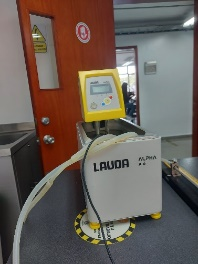
\includegraphics[width=3cm]{i1.jpg}
		\caption{Baño de termostatado.}
		\label{1}
		\end{figure}
  \item Dilatómetro: Se utiliza para registrar el cambio de longitud de la varilla
			 \begin{figure}[!h]
		\center
		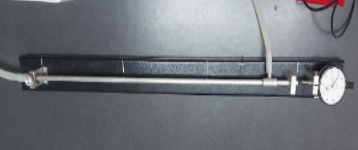
\includegraphics[width=6cm]{i2.png}
		\caption{Dilatómetro.}
		\label{2}
		\end{figure}
  \item Termómetro: Se utiliza para registrar los cambios de temperatura en el agua
			 \begin{figure}[!h]
		\center
		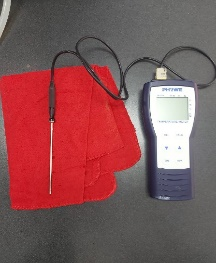
\includegraphics[width=4cm]{i3.jpg}
		\caption{Termómetro.}
		\label{3}
		\end{figure}
 \item Se utiliza para determinar la longitud inicial de la varilla
				 \begin{figure}[!h]
			\center
			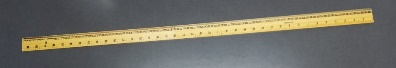
\includegraphics[width=6cm]{i4.jpg}
			\caption{Regla.}
			\label{4}
			\end{figure}


	\end{enumerate}

Primero para la recolección de datos con la ayuda del termómetro tomamos la temperatura del agua que tenemos en el baño de termostatado que tiene esa agua en contacto con el dilatómetro por medio de dos mangueras. A continuación, encendimos el baño de termostatado para que comenzara a calentar el agua hasta llegar a los 57,2 °C y comenzamos a tomar los datos del dilatómetro cada vez que el termómetro de contacto aumentaba 2°C, para poder calcular cual había sido la dilatación del dilatómetro, el coeficiente de dilatación lineal y la grafica de temperatura con respecto a el aumento de la longitud del dilatómetro.

\section{Objetivos}

\begin{enumerate}
	
    \item Explicar la expansión o dilatación de algunos cuerpos con el incremento de la temperatura
    
    \item Aplicar la teoría de la dilatación térmica para explicar hechos cotidianos.
    \item Medir el coeficiente de dilatación lineal de varillas de diferentes metales y hacer las gráficas de $\Delta L$ contra temperatura

	\end{enumerate}
%%%%%%%%%%%%%%%%%%%%%%%%%%MARCO TEÓRICO
\section{Marco Teórico}

 La dilatación térmica o expansión térmica es el aumento en las dimensiones de los cuerpos cuando se calientan.
La explicación del fenómeno reside en la agitación térmica de las partículas. De acuerdo a la teoría cinética, las moléculas que constituyen las sustancias no están en reposo, sino en movimiento permanente.
En los sólidos las partículas oscilan alrededor de un punto fijo, pero al aumentar la temperatura, la amplitud de la oscilación crece, y como consecuencia el objeto se expande.
 
 
 
\textbf{     TIPOS DE DILATACIÓN TÉRMICA}
 
 \begin{itemize}
    \item La más frecuente, que se da cuando el material aumenta simplemente sus dimensiones con la temperatura y se llama dilatación o expansión térmica.    
    \item Expansión térmica negativa, si la sustancia se encoge al calentarse.
\end{itemize}
	
	De acuerdo a las dimensiones predominantes en el objeto, la expansión térmica puede ser lineal, superficial o volumétrica.
	
 \subsection{Dilatación lineal}
El cambio en la longitud de una varilla, barra o alambre delgado se denota como $\Delta L$ y es directamente proporcional al cambio de temperatura $\Delta T$ ya la longitud original $L_{o}$:

\begin{figure}[!h]
		\center
		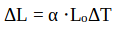
\includegraphics[width=3cm]{eq1.png}
		\caption{Dilatación Lineal}
		\label{1}
		\end{figure}
		
	Donde:
	
\begin{itemize}
    \item $\Delta L$ = Longitud final — Longitud inicial = $L_{f}$ — $L_{o}$
    \item $\Delta T$ = Temperatura final — Temperatura inicial = $T_{f}$ — $T_{o}$
    \item $\alpha$ es la constante de proporcionalidad, llamada coeficiente de 	expansión lineal, positivo si la longitud aumenta con la temperatura.
\end{itemize}
	
	Los valores de $\alpha$ para las diferentes sustancias, en unidades de inverso de temperatura, están tabulados, casi siempre a 20 ºC, aunque el valor se mantiene constante en un buen rango de temperaturas.
La ecuación anterior se puede reescribir para calcular directamente la longitud final:
	
	\begin{figure}[!h]
		\center
		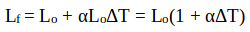
\includegraphics[width=5cm]{eq2.png}
		\caption{Longitud Final- DIlatación Lineal}
		\label{2}
		\end{figure}
		
		\begin{table}[!h]
\center
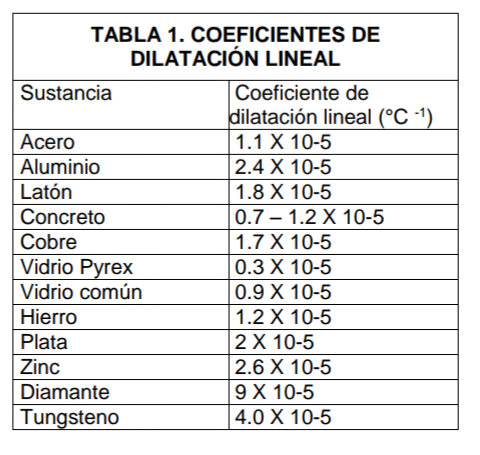
\includegraphics[width=8cm]{table1.png}
\caption{Coeficientes de dilatación lineal}
\label{T2}
\end{table}
		
		
		
\subsection{Dilatación Superficial}

	De manera análoga a la ecuación anterior, para una lámina con superficie inicial $S_{o}$ , se puede demostrar que la nueva superficie Sf viene dada por:
	\begin{figure}[!h]
		\center
		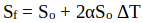
\includegraphics[width=3.5cm]{eq3.png}
		\caption{Dilatación Superficial}
		\label{3}
		\end{figure}
		
	\begin{table}[!h]
\center
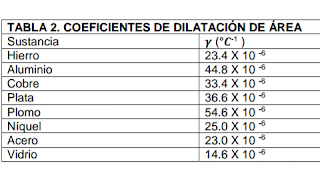
\includegraphics[width=8cm]{table2.png}
\caption{Coeficientes de dilatación superficial}
\label{T3}
\end{table}	


		\subsection{Dilatación Volumétrica}
	
	Finalmente, para un objeto de volumen inicial $V_{o}$ , el nuevo volumen $V_{f}$ es: 
	\begin{figure}[!h]
		\center
		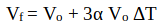
\includegraphics[width=3.5cm]{eq4.png}
		\caption{Dilatación VOlumétrica}
		\label{3}
		\end{figure}
		
	\begin{table}[!h]
\center
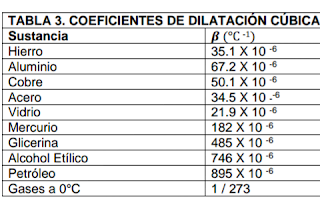
\includegraphics[width=8cm]{table3.png}
\caption{Coeficientes dilatación Volumétrica}
\label{T3}
\end{table}	
		
		En la vida cotidiana se presencian diferentes casos de dilatación térmica, como sucede con el aire contenido dentro de las ruedas de los autos, donde en verano al aumentar la temperatura se dilata aumentado su volumen, por lo que las ruedas de los autos quedan más infladas en verano que en invierno. Otra forma en que se presencia la dilatación térmica es el hecho de que generalmente muchos vasos de vidrio se quiebren ante cambios brusco de temperatura. La explicación es que el vidrio en la parte interior del vaso se dilata más rápidamente al estar en contacto con el líquido que en la parte de afuera, eso hace que se quiebre debido a que la parte exterior no logra dilatarse tan rápidamente.
		
		
	

 
%%%%%%%%%%%%%%%%%%%%%%%%%%METODOLOGIA
\section{Resultados} 

\subsection{DATOS REGISTRADOS} 

  

Con el fin de medir el coeficiente de dilatación lineal de 1 varilla de un material metálico, nos disponemos a hacer uso de los materiales mencionados anteriormente para realizar un montaje en el cual medimos la expansión lineal de la varilla que recibe transferencia de calor por sus extremos por medio de una conexión de mangueras a través de un baño termostatado que lleva agua caliente a los extremos de la varilla y por transferencia térmica, el calor del agua es transferido a la barra por sus dos extremos. Con la ayuda del dilatómetro registramos el cambio de la longitud de la varilla y con la ayuda de un Termómetro, medimos el cambio de la temperatura. Estos datos son registrados y tabulados en sus unidades originalmente medidas en la Tabla \ref{T4}, es decir, se muestra $\Delta L$  en milímetros (mm) y $\Delta T$  en grados Centígrados (°C), la temperatura fue registrada cada 2°C. 

  

\begin{table}[!h] 

\center 

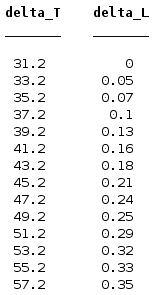
\includegraphics[width=4cm]{rawData.png} 

\caption{Datos registrados: Medidas del laboratorio} 

\label{T4} 

\end{table} 

  

El objetivo de este laboratorio fue principalmente determinar el coeficiente de dilatación lineal de la varilla, para darnos una idea del tipo d material que estamos manejando. Es por esto que utilizando la ecuación de dilatación lineal de la Figura \ref{1}, podemos buscar una relación lineal en nuestros datos, con el fin de buscar una línea de ajuste y determinar la pendiente, la cual corresponde a $\alpha$ o a el coeficiente de expansión lineal buscado. 

  

\subsection{GRAFICAS} 

  

Primero realizamos una gráfica de los puntos obtenidos en el laboratorio. esto con el fin de observar el comportamiento de los datos y ver si sería lógico realizar un ajuste lineal en estos. 

  

\begin{figure}[!h] 

\center 

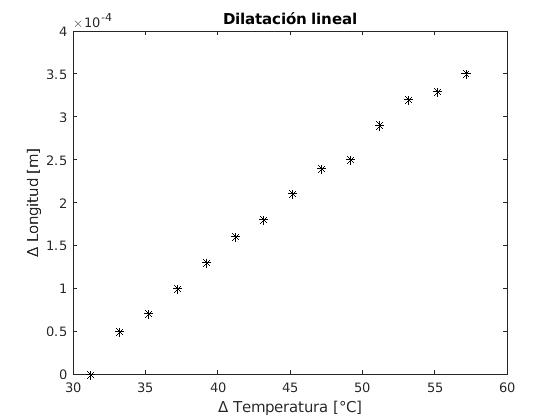
\includegraphics[width=10cm]{g1.jpg} 

\caption{Gráfica 1: Representación de los datos medidos (UNIDADES INTERNACIONALES)} 

\label{6} 

\end{figure} 

  

De la anterior gráfica, podemos decir que existe un comportamiento lineal como el esperado, es por esto que realizamos la siguiente gráfica donde ajustamos los datos a una línea recta, según la distancia que tienen estos puntos con respecto a su media elevado al cuadrado (mínimos cuadrados), utilizando una función de MATLAB®.  

  

\begin{figure}[!h] 

\center 

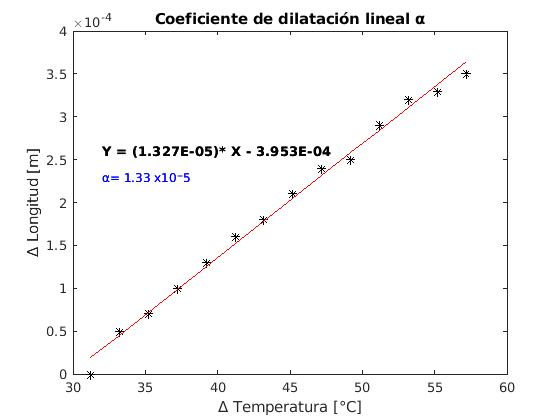
\includegraphics[width=10cm]{g2.jpg} 

\caption{Gráfica 2: Ajuste lineal, para encontrar $\alpha$ (UNIDADES INTERNACIONALES)} 

\label{6} 

\end{figure} 

  

De la gráfica podemos concluir entonces que le valor de buscado es $\alpha= 1.33E-5$ 
%%%%%%%%%%%%%%%%%%%%%%%%%%%%%%%%%%%%%%%%%%%%%%%%%%%%RESULTADOS

\section{Análisis de resultados}


Los datos del laboratorio se realizaron con la ayuda de un dilatómetro el cual poseía una precisión de 0.01 mm. Debido a la naturaleza de este experimento, no hemos podido realizar una repetición de los experimentos y solo contamos con una única medida para cada punto. Debido a esto, el error prominente en este laboratorio se deriva de los instrumentos de medición; del dilatómetro para registrar los cambios de longitud y del termómetro para registrar los cambios de Temperatura. EL error debido al operador en este caso fue mucho menor, ya que su labor se limitó únicamente a registrar los valores dados por los instrumentos electrónicos, y debido a que había 4 personas realizando las observaciones, podemos decir que en este aspecto el error fue el menor posible. 

  

De esta forma, los datos registrados en el laboratorio fueron posteriormente graficados y se realizó la regresión lineal para calcular la pendiente que representa el coeficiente de expansión lineal $\alpha $. De esto, obtuvimos un valor de $\alpha= 1.33E-5$ .  

  

De antemano, intuimos que el material trabajado es una especie de metal, que podría ser desde acero, hierro, aluminio. Sin embargo, debido a su gran peso, podríamos descartar el aluminio. Por lo tanto, podríamos intuir que el material experimental es un tipo de acero o es simplemente hierro. Sin embargo, debido a sus características de su superficie, el material parecía ser una aleación de hierro, es decir un acero, más que ser puro hierro. Para determinar con mayor precisión que tipo de material es, procedemos a comparar el valor de la pendiente obtenida en la Gráfica 2 (Figura \ref{6}) ($\alpha= 1.33E-5$), con los datos que se presentan en la Tabla \ref{T2}. 

  

De allí podemos observar que   para el Acero: ($\alpha= 1.1E-5$), para el Hierro :($\alpha= 1.2E-5$). Por lo tanto, podemos decir que nuestro material esta más próximo al HIERRO. que al acero. 

  

Por otro lado, como se mencionó el ajuste de los datos se realizó utilizando una función que minimiza el error cuadrático medio con el fin de encontrar un ajuste lineal de los 2 coeficientes (pendiente e intercepto eje y) que presenten una distancia menor a su media como sea posible. Sin embargo, no es la única forma de ajustar este tipo de datos, hoy en día existen muchos tipos de ajustes lineales y modelos de regresión lineal, que se basan en diferentes aproximaciones para encontrar un ajuste lineal coherente. Sin embargo, podemos decir que con las técnicas utilizadas en este laboratorio fue posible determinar que el material trabajado era Hierro.  


\section{Conclusion}
	
	\begin{enumerate}[label=(\roman*)]
	
    \item Como se observó en la práctica y junto al marco teórico estudiado para realizar el trabajo, notamos que la temperatura influye en las magnitudes de los cuerpos que se están estudiando, en el caso de aumentar la temperatura, el cuerpo va a aumentar una de sus magnitudes, en el caso de nuestro experimento notamos que al aumentar la temperatura la longitud de la barra aumentó y el radio de la barra disminuyó. Mientras que, si dejábamos que la temperatura disminuyera, la barra iba a contraerse e iba a disminuir sus medidas.
    \item  Se observó que la dilatación térmica es algo muy común en nuestra vida diaria, por ejemplo podemos aplicarla cuando nos ponemos unos zapatos que nos quedan precisos por la mañana y al terminar el día notamos que estos están un poco más sueltos, esto debido al aumento de temperatura que tuvo el objeto de estudio
    
    \item  Los materiales se expanden y se contraen según su cambio de temperatura y la naturaleza del material. Este laboratorio nos permitió verificar la expansión lineal de una varilla y nos muestra la importancia de tener en cuenta la física, como en este caso la dilatación térmica de los materiales, cuando nos encontramos realizando diseños a problemas de ingeniería.  
    


	\end{enumerate}

\appendices


\ifCLASSOPTIONcaptionsoff
  \newpage
\fi


\begin{thebibliography}{1}


 \bibitem{IEEEhowto:Monteria}
  Fanny Zapata. (10 de mayo de 2021). Dilatación térmica. Lifeder. Recuperado de: https://www.lifeder.com/dilatacion-termica/. 

 \bibitem{IEEEhowto:Monteria}
 La química y nosotros  (4 de Junio de 2013) Dilatación térmica en la vida cotidiana. Recuperado de: $http://katherinevaleria21.blogspot.com/2013/06/dilatacion-termica-en-la-vida-cotidiana_4.html $
\end{thebibliography}



\end{document}
